%
%
% SUMMARY:
% USAGE:
%
% AUTHOR:       Christophe Prud'homme
% ORG:          Christophe Prud'homme
% E-MAIL:       prudhomm@zion
%
% ORIG-DATE:  7-Apr-04 at 16:48:32
% LAST-MOD:  7-Apr-04 at 23:07:19 by Christophe Prud'homme
%
% DESCRIPTION:
% DESCRIP-END.

\documentclass[11pt,a4paper]{article}
\usepackage[]{times}
\usepackage{fullpage}
\addtolength{\textheight}{1cm}
\usepackage[pdftex]{graphicx}
\usepackage{subfigure}
\usepackage{amsmath}
\usepackage{xspace}
\usepackage{color}

\usepackage{floatflt}

\usepackage{indentfirst}
\usepackage{amssymb}
\usepackage{url}
\usepackage{bm}
\usepackage{multirow}


\usepackage{svninfo}
\usepackage{fancyhdr}
\pagestyle{fancyplain}
\fancyhead[RE,LO]{\leftmark}
\fancyhead[LE,RO]{\thepage}

\usepackage[bookmarks=true,bookmarksopen=true,breaklinks=true,colorlinks=true,citecolor=blue,linktocpage=true]{hyperref}

\newcommand{\abs}[1]{\biggl| #1 \biggr|}
\newcommand{\jump}[1]{[\![#1]\!]}
\newcommand{\paren}[1]{\left(#1\right)}
\newcommand{\prect}[1]{\left[#1\right]}
\newcommand{\norm}[1]{\Vert#1\Vert}
\newcommand{\set}[1]{\{#1\}}



\newcommand{\domain}{\Omega}
\newcommand{\boundary}{\partial \domain}

\newcommand{\ltwo}{L^2(\domain)}
\newcommand{\ltwozero}{L^2_0(\domain)}
\newcommand{\hs}[1]{ {\textbf H^{#1}(\domain)}}
\newcommand{\hone}{\hs{1}}
\newcommand{\honezero}{\textbf H^1_0(\domain)}

\newcommand{\poly}[2]{\mathbb P_{#1}#2}
\newcommand{\qoly}[2]{\mathbb Q_{#1}#2}
\newcommand{\cO}{\mathcal{O}}
\newcommand{\cT}{\mathcal{T}}
\newcommand{\Poly}{\mathbb{P}}


%\newcommand{\IR}{{\,\mathbb{R}\,}}
\newcommand{\IR}{I\!\!R}
%\newcommand{\N}{{\,\mathbb{N}\,}}
\newcommand{\IN}{I\!\!N}

\newcommand{\matr}[1]{\mathbf{#1}}
\renewcommand{\vec}[1]{\boldsymbol{#1}}
\newcommand{\Matr}[2]{\left(\begin{array}{#1} #2 \end{array} \right)}
\newcommand{\vvec}[3]{\Matr{#1}{#2 \\ #3}}
\newcommand{\vvvec}[4]{\Matr{#1}{#2 \\ #3 \\ #4}}
\newcommand{\vvecT}[3]{\left(#2,#3 \right)^{\top}}
\newcommand{\vvvecT}[4]{\left(#2,#3,#4 \right)^{\top}}

\newcommand{\Nabla}{\vec{\nabla}}
\newcommand{\grad}{\Nabla}
%\newcommand{\grad}{\mathrm{grad}}
\renewcommand{\div}{\Nabla\cdot}
%\renewcommand{\div}{\mathrm{div}}

\newcommand{\dd}{\mathrm{d}}

\newcommand{\That}{\ensuremath{\hat{T}}}
\newcommand{\Nel}{\ensuremath{{N_{\mathrm{el}}}}}
\newcommand{\geo}{\ensuremath{{\mathrm{geo}}}}
\newcommand{\Ngeo}{\ensuremath{{N_{\geo}}}}
\newcommand{\bphi}{\ensuremath{\vec{\varphi}}}
\newcommand{\PS}[1]{\ensuremath{\mathbb{P}_{#1}}}
\newcommand{\vdisp}{\ensuremath{\vec{d}}}
\newcommand{\vforce}{\ensuremath{\vec{f}}}

\newcommand{\eref}[1]{(\ref{#1})}

\date{}%leave empty

\newcommand{\cpp}{{\sl\sffamily
C{\kern-.0em\lower+.4ex\hbox{$^{\text{\sl\sffamily ++}}$}}}\xspace}


\title{Flow around a cylinder}
\author{}
\date{}

\begin{document}

\maketitle
\thispagestyle{empty}

\section{Introduction}

Sch\"afer and Turek provide in \cite{schaefer:1996} the definition of
a series of test cases involving two and three dimensional laminar
flow around a cylinder, along with reference values for some benchmark
quantities, established by comparison of results of different research
groups.


We consider that the flow is \emph{isothermal}. We now denote the
following quantities:
\begin{itemize}
\item $d$ the geometric dimension with $d=2$ or $d=3$
\item $\vec{u}$ the velocity
\item $p$ the pressure
\item $\rho$ the density
\item $\mu$ the dynamic viscosity. The SI physical unit of dynamic
  viscosity is the pascal-second ($Pa\cdot s$), which is identical to $1
  kg\cdot m^{-1} \cdot s^{-1}$.
\item $\vec{f}$ the volumic force applied to the fluid which are
  neglected in our case, \emph{i.e.} $\vec{f} = \vec{0}$
\item  $\varepsilon(\vec{u})$ the strain rate tensor. It reads
\begin{equation}
  \label{eq:3}
  \mathbb{\varepsilon}(\vec{u}) = \frac{1}{2} \Big( \nabla \vec{u} + \big( \nabla \vec{u} \big)^T \Big)
\end{equation}
\item $\mathbb{D}( \mu )$ the total stress tensor for a Newtonian fluid
\begin{equation}
  \label{eq:2}
  \mathbb{D}( \vec{u} ) = -p \mathbb{I} + 2 \mu \mathbb{\varepsilon}(\vec{u})
\end{equation}
where $\mathbb{I}$ denotes the identity matrix of size $d \times d$

\end{itemize}



We look for the pair velocity/pressure $(\vec{u}, p)$ in $\Omega$ that
solve
  \begin{eqnarray}
    \rho \frac{\partial \vec{u} }{\partial t} + \rho \nabla \cdot \big( \vec{u} \otimes \vec{u} \big) - \nabla \cdot \big(  \mathbb{D} (\vec{u}) ) & = \displaystyle\vec{f}   \label{eq:1}\\
    \nabla \cdot \vec{u} & =  0 \label{eq:7}
  \end{eqnarray}

which also reads
\begin{eqnarray}
  \rho \frac{\partial \vec{u} }{\partial t} + \rho \vec{u} \cdot \nabla \vec{u}\ -\ \mu \Delta \vec{u}\ +\ \nabla p  & = \vec{f}   \label{eq:5}\\
  \nabla \cdot \vec{u} & = 0\label{eq:6}
\end{eqnarray}




\subsection{Definition of the Test Cases}

\subsubsection{Problem Setting}

We consider here the test cases 2D-1 and 3D-Z1 from \cite{schaefer:1996}.
The Navier-Stokes equations \eref{eq:ns_strong}, \eref{eq:div_strong} are solved on a domain $\Omega\subset\IR^{d}$, $d\in{2,3}$.
For the test case 2D-1, we have $d=2$ and the domain $\Omega$ is given by Figure \ref{fig:cyl_geom_2d}.
\begin{figure}[!htbp]
\begin{center}
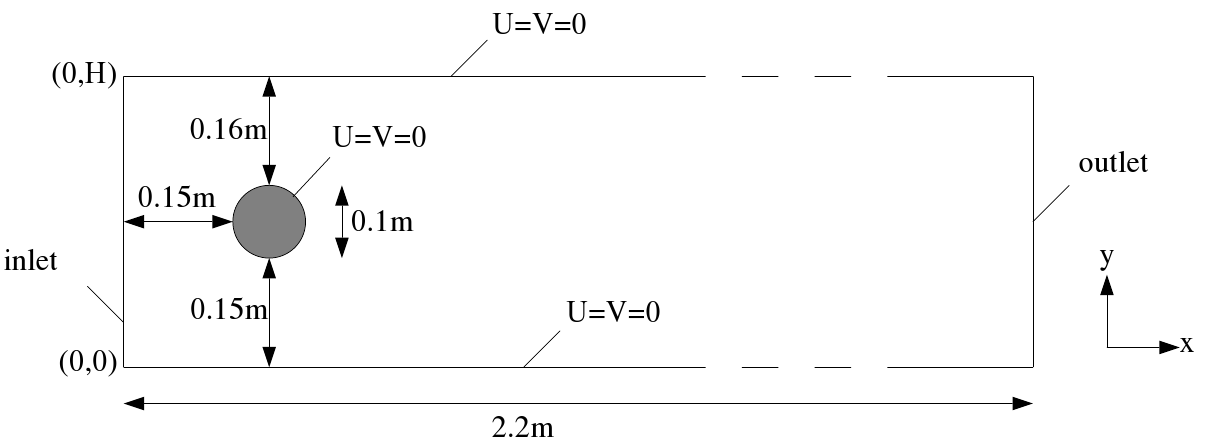
\includegraphics[width=0.75 \textwidth]{figures/cylinder2d_geom}
\caption{2D cylinder benchmark flow - geometry}
\label{fig:cyl_geom_2d}
\end{center}
\end{figure}
For the test case 3D-Z1, we have $d=3$ and the domain $\Omega$ is given by Figure \ref{fig:cyl_geom_3d}.
\begin{figure}[!htbp]
\begin{center}
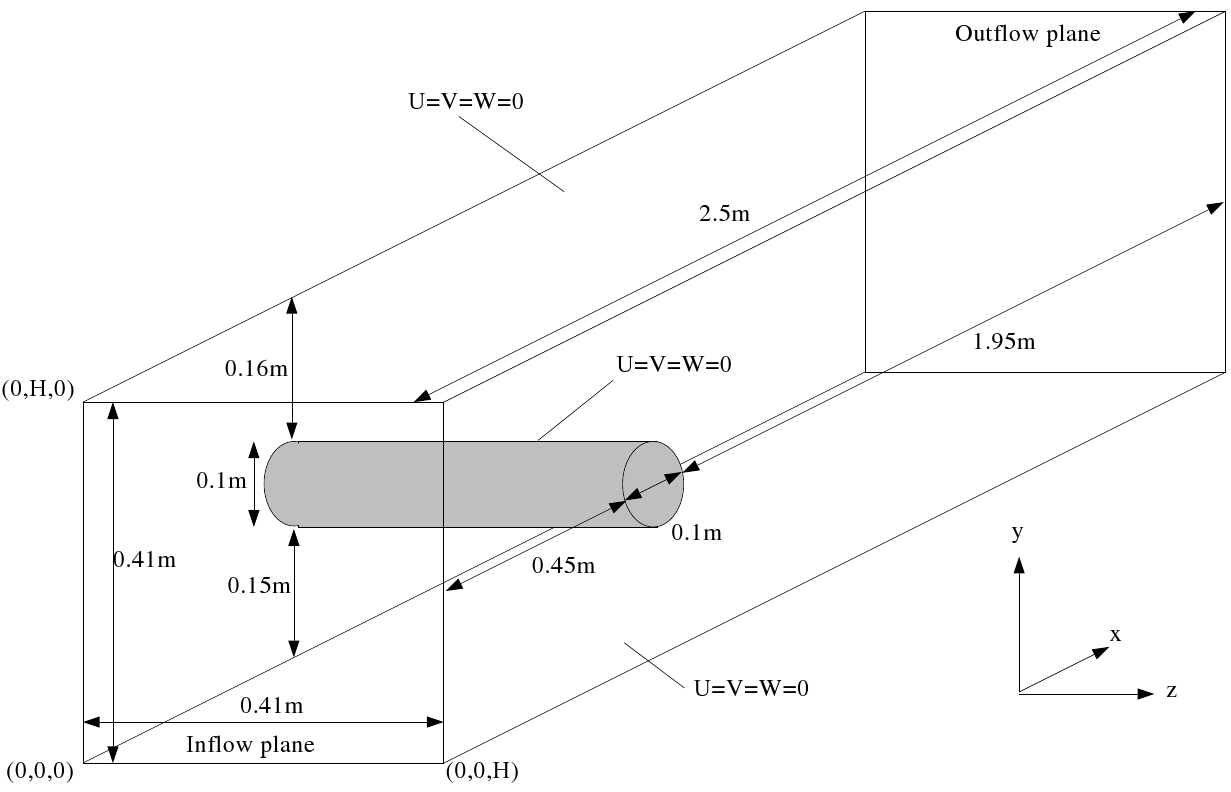
\includegraphics[width=0.75 \textwidth]{figures/cylinder_geom}
\caption{3D cylinder benchmark flow - geometry}
\label{fig:cyl_geom_3d}
\end{center}
\end{figure}
The density is $\rho=1.0\mbox{ kg}/\mbox{m}^3$ and the viscosity is
$\mu=10^{-3}\mbox{ Pa s}$, both constant throughout in time and space.
We denote by $H$ the channel height (and width) $H=0.41\mbox{ m}$ and
by $D$ the cylinder diameter $D=0.1\mbox{ m}$.

On the inflow section, Dirichlet boundary conditions are imposed, with
\begin{align*}
%%%%%%%%%%%%%%%%%%%%%%%%%%%%%%%%%%%%%%%%%%%%%%%%%%%%%%%%%%%%%%%%%%%%%%%%%%%%%%%%
   \vec{g}_D
&= \vvecT{c}{4 U_m x_2 (H-x_2) / H^2}{0}
& &\mbox{and} &
   U_m
&= 0.3\mbox{ m/s}
& &\mbox{for} &
   d=2
,\\
%%%%%%%%%%%%%%%%%%%%%%%%%%%%%%%%%%%%%%%%%%%%%%%%%%%%%%%%%%%%%%%%%%%%%%%%%%%%%%%%
   \vec{g}_D
&= \vvvecT{c}{16 U_m x_2 (H-x_2) x_3 (H-x_3) / H^4}{0}{0}
& &\mbox{and} &
   U_m
&= 0.45\mbox{ m/s}
& &\mbox{for} &
   d=3
,
%%%%%%%%%%%%%%%%%%%%%%%%%%%%%%%%%%%%%%%%%%%%%%%%%%%%%%%%%%%%%%%%%%%%%%%%%%%%%%%%
\end{align*}
where $U_m$ denotes the maximal inflow velocity.  The average inflow
velocity is then $\bar{U}=(\frac{2}{3})^{d-1}U_m=0.2\mbox{ m/s}$ in
both dimensions, which gives a Reynolds number of
$Re=\rho\bar{U}D/\mu=20$.  At this Reynolds number, the flow is
stationary.  On the outflow section, the benchmark description
\cite{schaefer:1996} leaves free choice of boundary conditions.  We
choose to apply homogeneous Neumann boundary conditions on the outflow
section.  On the rest of the boundary, homogeneous Dirichlet boundary
conditions are imposed.


\subsubsection{Benchmark Quantities}

The three benchmark quantities are the drag coefficient $c_D$, the
lift coefficient $c_L$ and the pressure difference $\Delta p$.  For
the drag and lift coefficients, we compute the force on surface $S$ of
the cylinder, shaded in grey in figures \ref{fig:cyl_geom_2d}
and \ref{fig:cyl_geom_3d}.  The cylinder force $\vec{F}_S$ is given by
\begin{equation*}
  \vec{F}_S
= \int_{S}\left( 2\mu\varepsilon(\vec{u})\cdot\vec{n} - p\vec{n} \right) \dd S.
\end{equation*}
We note $\vec{F}_S=\vvecT{l}{F_D}{F_L}$ for $d=2$ and
$\vec{F}_S=\vvvecT{l}{F_D}{F_L}{F_z}$ for $d=3$, where $F_D$ is the
drag force and $F_L$ is the lift force.  The drag and lift
coefficients $c_D$ and $c_L$ are:
\begin{equation*}
  c_D = \frac{2 F_D}{\rho\bar{U}^2 D H^{d-2}}
  \quad\mbox{and}\quad
  c_L = \frac{2 F_L}{\rho\bar{U}^2 D H^{d-2}}.
\end{equation*}

The pressure difference is the difference of the pressure between a point $\vec{x}_a$ before and a point $\vec{x}_e$ after the cylinder:
\begin{equation*}
  \Delta p=p(\vec{x}_a)-p(\vec{x}_e)
,
\end{equation*}
where
\begin{align*}
%%%%%%%%%%%%%%%%%%%%%%%%%%%%%%%%%%%%%%%%%%%%%%%%%%%%%%%%%%%%%%%%%%%%%%%%%%%%%%%%
   \vec{x}_a
&= \vvecT{l}{0.15}{0.20}\mbox{ m}
& &\mbox{and} &
   \vec{x}_e
&=  \vvecT{l}{0.25}{0.20}\mbox{ m}
& &\mbox{for } d=2, \mbox{ and}\\
%%%%%%%%%%%%%%%%%%%%%%%%%%%%%%%%%%%%%%%%%%%%%%%%%%%%%%%%%%%%%%%%%%%%%%%%%%%%%%%%
   \vec{x}_a
&= \vvvecT{l}{0.45}{0.20}{0.205}\mbox{ m}
& &\mbox{and} &
   \vec{x}_e
&= \vvvecT{l}{0.55}{0.20}{0.205}\mbox{ m}
& &\mbox{for } d=3.
%%%%%%%%%%%%%%%%%%%%%%%%%%%%%%%%%%%%%%%%%%%%%%%%%%%%%%%%%%%%%%%%%%%%%%%%%%%%%%%%
\end{align*}


\subsection{Evaluation of the Benchmark Quantities}

The integrals for the drag and lift forces are evaluated by numerical
integration of the stress on the cylinder surface.  This approach has
been analyzed in \cite{tabata:1998}.  An alternative approach, first
used in \cite{john:2002} and explained in more detail in
\cite{braack:2005}, consists in transforming the surface integrals
into integrals over the whole domain.  It turns out that the integral
forces are simply given by the bilinear form of the finite element
method \emph{without boundary terms}, evaluated for $(\vec{u},p)$ the
solution in consideration and tested with $(\vec{v},q)$ such that
$\vec{v}$ is the unit vector in the direction of interest on the part
of the boundary of interest $S$ and zero on the rest of the boundary,
and $q=0$.  This approach has been extended to the case of stabilized
finite element methods in \cite{braack:2004}.

Note that unlike in two dimensions, the cylinder surface $S$ touches
the rest of the boundary $\partial\Omega\setminus S$ in three
dimensions.  In order to apply the domain integral approach, the test
function should then be discontinuous and therefore cannot be in the
continuous finite element space.  So either the domain integral has to
be computed without using the matrix, which makes it way more
expensive than surface integration, or the test function has to be
approximated in the finite element space, which introduces additional
errors.  We therefore prefer the straightforward integration of the
stress on the cylinder surface.




\bibliographystyle{plain}
\bibliography{report}
\end{document}



%%% Local Variables:
%%% coding: utf-8
%%% mode: latex
%%% TeX-PDF-mode: t
%%% TeX-parse-self: t
%%% x-symbol-8bits: nil
%%% TeX-auto-regexp-list: TeX-auto-full-regexp-list
%%% TeX-master: t
%%% ispell-local-dictionary: "french"
%%% End:
